%% ============================================================================
%% §5 Design Optimizations  --  ASIC + FPGA each writes own subsection
%% ============================================================================
\section{Design Optimizations}
\label{sec:opt}

\subsection{ASIC Optimization Journey (Liao)}
\label{sec:opt:asic}

The ASIC implementation went through three architectural generations and four micro-architectural rounds. Each iteration was driven by a measurable shortfall in throughput, power, or area observed at the prior signoff. Figure~\ref{fig:evol_floorplans} shows the post-route floorplan for each generation; Table~\ref{tab:arch_evol} quantifies the metrics behind them.

\begin{figure}[H]
  \centering
  \begin{subfigure}{0.31\textwidth}
    \centering
    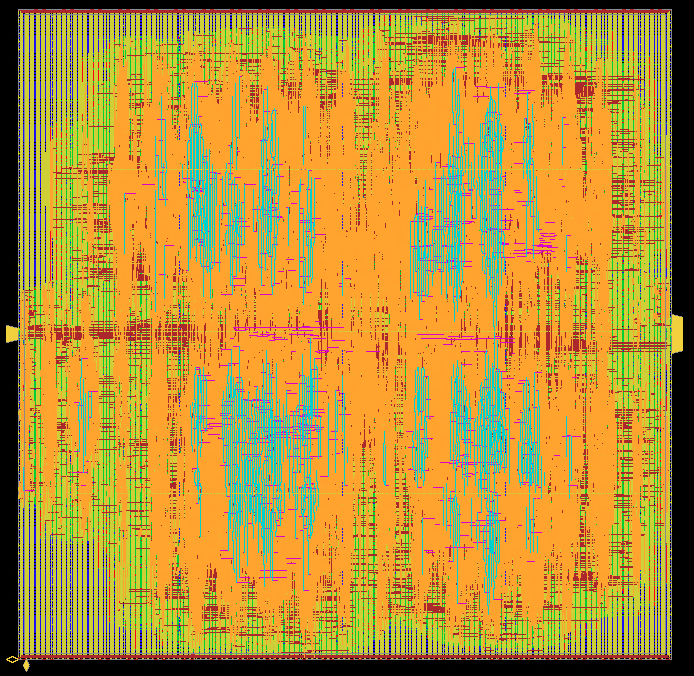
\includegraphics[width=\linewidth]{Fig/mfn_v1_pr.png}
    \caption{v1: 1$\times$9-MAC.}
    \label{fig:evol_v1}
  \end{subfigure}
\hfill
  \begin{subfigure}{0.31\textwidth}
    \centering
    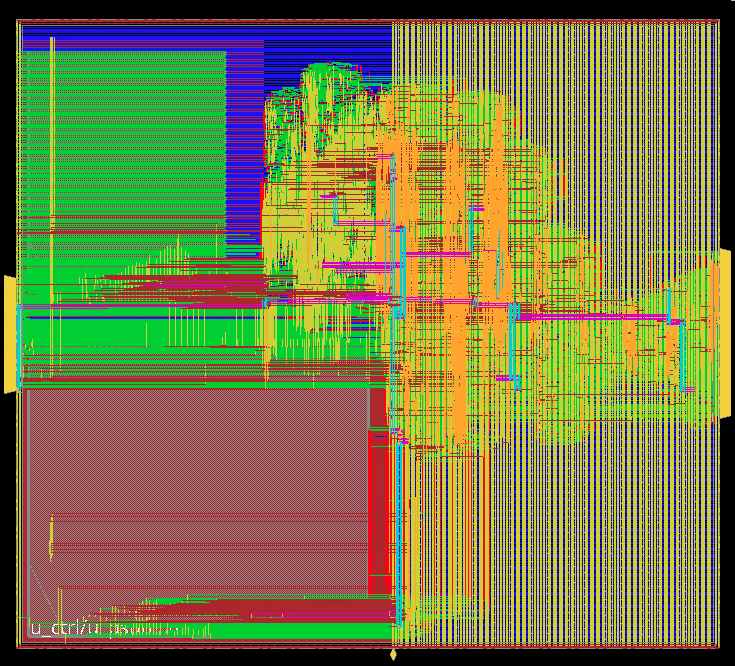
\includegraphics[width=\linewidth]{Fig/mfn_v2_pr.png}
    \caption{v2: 2$\times$9-MAC + psum SRAM.}
    \label{fig:evol_v2}
  \end{subfigure}
\hfill
  \begin{subfigure}{0.31\textwidth}
    \centering
    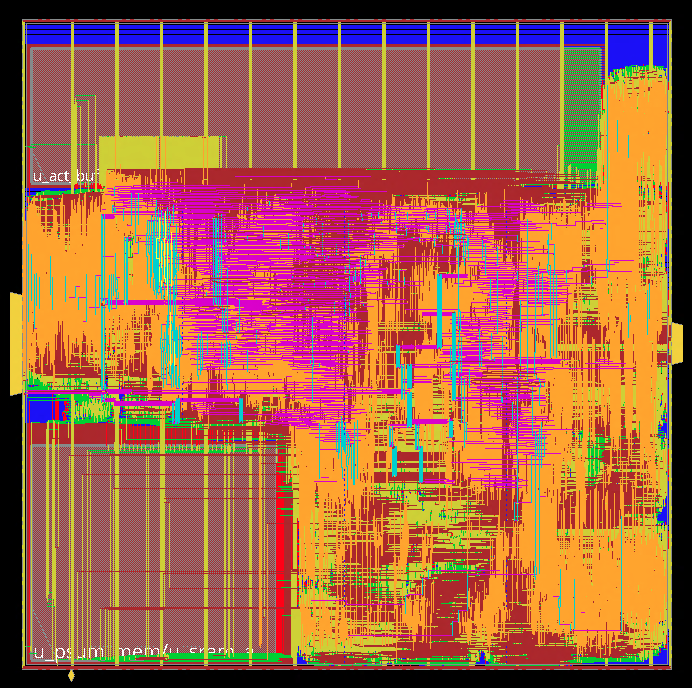
\includegraphics[width=\linewidth]{Fig/mfn_v3_pr.png}
    \caption{v3: 12$\times$12 SA + 2 SRAMs.}
    \label{fig:evol_v3}
  \end{subfigure}
  \caption[Post-route floorplan evolution v1 $\to$ v2 $\to$ v3.]{ ASIC architecture evolution: post-route floorplans for v1, v2, and v3. Visible progression from a single MAC datapath (v1) to a dual-MAC datapath with one OpenRAM macro (v2) to a $12\times12$ systolic array with two OpenRAM macros (v3, the final design).}
  \label{fig:evol_floorplans}
\end{figure}

\begin{figure}[H]
  \centering
  \begin{subfigure}{0.48\textwidth}
    \centering
    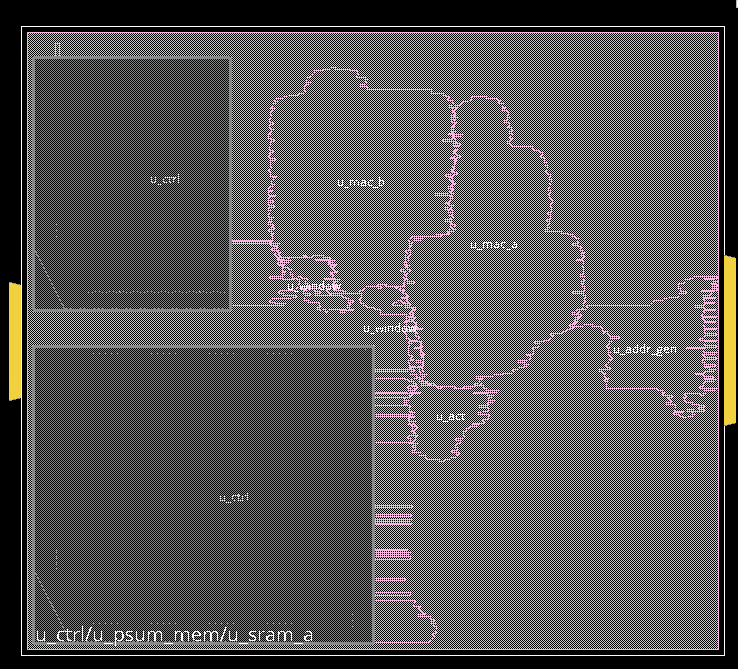
\includegraphics[width=\linewidth]{Fig/mfn_v2_pr_part.png}
    \caption{v2 detail: psum SRAM macro placed bottom-left.}
    \label{fig:v2_detail}
  \end{subfigure}
\hfill
  \begin{subfigure}{0.48\textwidth}
    \centering
    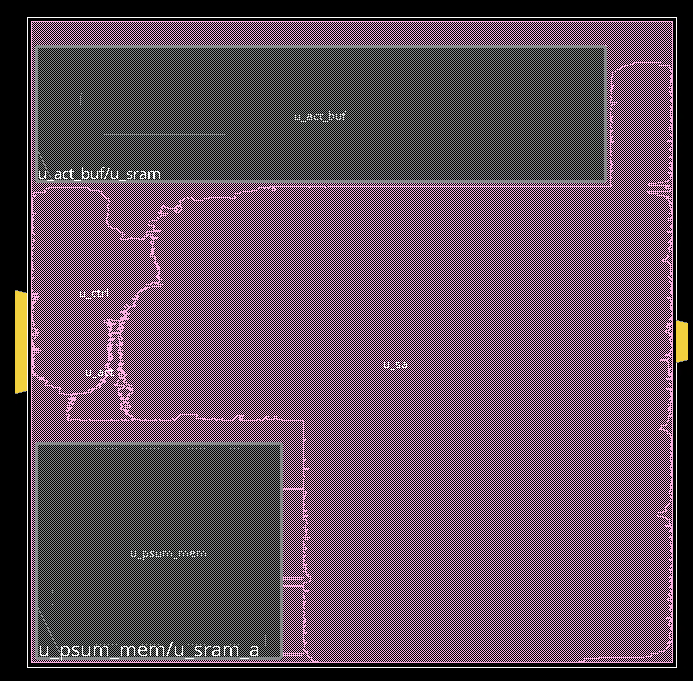
\includegraphics[width=\linewidth]{Fig/mfn_v3_pr_part.png}
    \caption{v3 detail: act\_buf and psum SRAM macros bracket the SA.}
    \label{fig:v3_detail}
  \end{subfigure}
  \caption[Macro placement evolution v2 $\to$ v3.]{Macro placement evolution v2 $\rightarrow$ v3.}
  \label{fig:v2_v3_detail}
\end{figure}

\begin{table}[H]
\centering
\caption{ASIC Architecture Evolution: v1 $\to$ v2 $\to$ v3}
\label{tab:arch_evol}
\begin{tabularx}{\textwidth}{l X X X}
\toprule
\headrow & \textbf{v1} & \textbf{v2} & \textbf{v3 (final)} \\
\midrule
Compute        & single 9-MAC dot-product       & dual 9-MAC (18 mult, 2 out-ch parallel) & 12$\times$12 = 144-MAC SA           \\
Adder          & 38-stage ripple carry          & 40-bit 2-level CLA & CLA + Stage 3 SA pipeline           \\
psum memory    & 512$\times$40 FF              & + OpenRAM SRAM macro (psum) & + OpenRAM SRAM macro (1RW+1R)       \\
act memory     & FF array                       & FF array & + OpenRAM SRAM macro (192$\times$64)\\
Cycles / inf   & 43.16\,M                       & 25.77\,M                            & 13.77\,M  \\
Clock          & 100\,MHz                       & 125\,MHz                            & 200\,MHz  \\
FPS            & 2.3                            & 4.85                                & 14.5      \\
Power          & 26.7\,mW                       & 11.4\,mW                            & 96.3\,mW  \\
Core area      & $\sim$285\,K $\mu$m$^2$        & 479\,K $\mu$m$^2$                   & 518\,K $\mu$m$^2$ \\
DRC            & 0                              & 0                                   & 0 \\
\bottomrule
\end{tabularx}
\end{table}

v1's single 9-MAC unit produced one output channel per cycle, so 8/9 of the available parallelism was wasted on pointwise layers. v2 doubled the MAC count to 18 (two parallel output channels) and replaced the 38-stage ripple-carry adder with a 40-bit two-level CLA. The biggest win was moving the 512$\times$40 psum memory from an FF array into an OpenRAM SRAM macro: total cell count dropped and post-route power fell from 26.7\,mW to 11.4\,mW even though the MAC count had doubled.

v3 then generalised to a $12\times12 = 144$-MAC output-stationary systolic array (\texttt{mfn\_sa\_12x12}), each PE holding a 40-bit accumulator. The cycle count roughly halved again (25.77\,M to 13.77\,M). Power rises to 96.3\,mW because 144 multipliers now toggle every cycle at 200\,MHz; the meaningful figure of merit is energy per inference, which lands at 6.63\,$\mu$J.

Within v3, four cumulative micro-optimizations were applied (Table~\ref{tab:v3_opt}). Each was driven by the previous round's WNS report or power breakdown.

\begin{table}[H]
\centering
\caption{v3 Cumulative Micro-Optimizations}
\label{tab:v3_opt}
\begin{tabularx}{\textwidth}{l X l l l}
\toprule
\headrow \textbf{Round} & \textbf{Change} & \textbf{$F_{max}$} & \textbf{FPS} & \textbf{Power} \\
\midrule
Baseline (2-stage activation)  & Stage 0+1 only           & 87\,MHz  & 6.0  & 45.4\,mW \\
+ Stage 0+2 split              & Lane-select pipelined    & 150\,MHz & 10.9 & 77.9\,mW \\
+ Stage 3 SA \texttt{row\_dot\_reg} & $\mathit{acc+row\_dot}$ split off & 174\,MHz & 12.6 & 88.2\,mW \\
+ 5.0\,ns push                 & $T_{clk}$ tightened only         & 200\,MHz & 14.5 & 99.1\,mW \\
+ 720$\times$720 area shrink   & smaller die, denser placement    & 200\,MHz & 14.5 & 96.3\,mW \\
\bottomrule
\end{tabularx}
\end{table}

Two non-architectural fixes were also required to reach signoff. The first is a LEF patch: the OpenRAM-emitted SRAM LEF reserves the whole of metal-3 and metal-4 as obstructions on every macro, but the read-data pins sit on metal-3, so the router has no legal via-3 escape and is forced to cross the obstructions. Without the patch the design reports $\sim$480 SHORT/SPACING DRC violations. The script \texttt{fix\_sram\_lef.py} removes the M3/M4 \texttt{OBS} blocks (the OpenRAM behavioural macros do not actually route on those layers) and snaps off-grid \texttt{RECT} and \texttt{SIZE} coordinates to the 0.005\,$\mu$m manufacturing grid. After patching, P\&R is DRC-clean.

The second is a testbench race. The first 50-layer post-route gate-level simulation reported all 50 layers as mismatches even though RTL was 50/50 MATCH. A \texttt{bind}-based probe localised the cause to the testbench: \texttt{pixel\_in} was driven on \texttt{@(posedge clk)} from the address the DUT presented on \texttt{x\_out}, but the gate-level netlist adds delta-cycle delay on port outputs, so the testbench latched the previous-cycle address. Driving on \texttt{@(negedge clk)}, after \texttt{x\_out} has settled, restored all 50 layers to exact match.

\subsection{FPGA Optimization (Zhang)}
\label{sec:opt:fpga}

% TODO friend: describe FPGA-side optimizations.
% Examples to cover (drop any that don't apply):
%   - Resource sharing (multi-cycle multiply on DSP)
%   - Pipelining of long combinational paths to hit Fmax
%   - URAM vs BRAM choice
%   - Burst-length tuning of AXI-Stream DMA
%   - HLS pragmas (UNROLL, ARRAY_PARTITION) if HLS path used
%   - Clock-gating or partial reconfiguration

\noindent\fbox{\parbox{\textwidth}{\itshape \textbf{Placeholder} --- Zhang's FPGA optimization narrative goes here, mirroring the structure of Section~\ref{sec:opt:asic}: quantitative ``before $\to$ after'' for each optimization (Fmax, resource use, throughput).}}
